\documentclass[12pt]{scrartcl}
\usepackage{config}
\usepackage{minted}

%\newcommand\mrh{\color{white}\bfseries}
\newcommand\mrc[1]{\begin{tabular}{@{}l@{}} #1 \end{tabular}}
\setlength\arrayrulewidth{0.8pt}

\usemintedstyle{pastie}

\begin{document}
    \hh{Determine Edges}
    
    \vspace{10pt}

    \hh{Problem}
    
        You are given an integer $N$ and $N - 1$ bidirectional edges. These edges connect $N$ vertices in such a way that there exists a path\footnote{Sequence of vertices such that any two adjacent vertices belong to an edge of the graph.} between any two vertices (i.e., they form a tree). You must assign weights to each of the edges such that the following property holds in the tree:
        
        For every integer $x$ between $1$ and $\left\lfloor \frac{2N^2}{9} \right\rfloor$, there exists a pair of vertices $i, j$ such that the sum of the weights on the simple path\footnote{That does not repeat edges.} between $i$ and $j$ is equal to $x$.
    
    \hh{Implementation Details}

        You must implement the function \textit{Determinar\_aristas()}. This function receives an integer $N$ and two vectors $u$ and $v$, each with $N - 1$ elements. For each $0 \le i \le N - 2$, $u[i]$ and $v[i]$ are the vertices connected by edge $i$. This function must return a vector with $N - 1$ elements, the weights you chose.
        The function would look like this:

\begin{minted}{c++}
#include <bits/stdc++.h>
using namespace std;

vector<int> Determinar_aristas(int N, vector<int> u, vector<int> v) {
    // Implement this function.
}
\end{minted}

    The grader will run the function \textbf{multiple} times for each test case.

    \hh{Example}
    
        {\itshape Example 1:}
        \begin{itemize}
            \item The grader calls the function 
            \begin{center}
                \textit{Determinar\_aristas(6, \{0, 1, 2, 2, 1\}, \{1, 2, 3, 4, 5\})}
            \end{center}
            the tree in this case is as follows:
            \begin{center}
                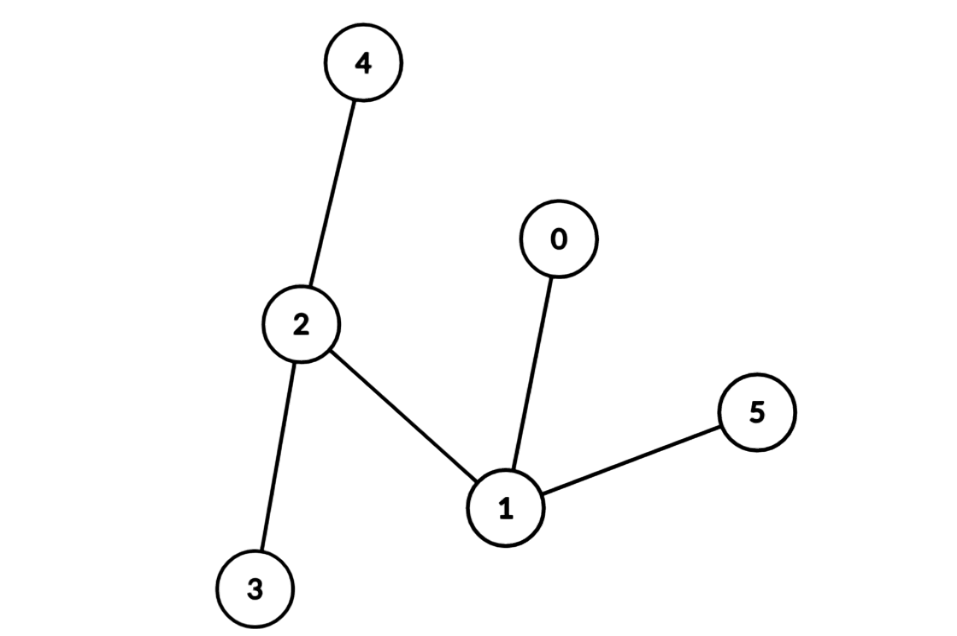
\includegraphics[scale=0.25]{ej1.png}
            \end{center}
            \item You could obtain the full points for this case by returning the vector \{2, 1, 2, 4, 5\}. Which corresponds to the following choice of edges:
            \begin{center}
                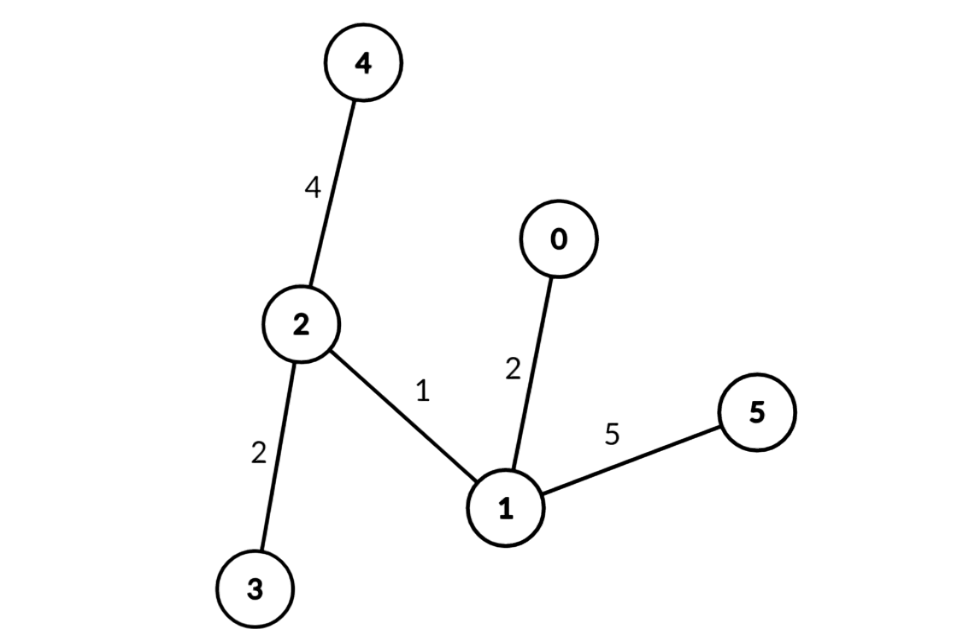
\includegraphics[scale=0.25]{ej2.png}
            \end{center}
            This is because:
            \begin{itemize}
                \item The path between vertices $(1, 2)$ has a weight of 1.
                \item The path between vertices $(0, 1)$ has a weight of 2.
                \item The path between vertices $(0, 2)$ has a weight of 3.
                \item The path between vertices $(2, 4)$ has a weight of 4.
                \item The path between vertices $(1, 5)$ has a weight of 5.
                \item The path between vertices $(2, 5)$ has a weight of 6.
                \item The path between vertices $(0, 5)$ has a weight of 7.
                \item The path between vertices $(3, 5)$ has a weight of 8.
            \end{itemize}
        \end{itemize}

    \hh{Constraints}
        \begin{itemize}
            \item $1 \le N \le 2000$.
            \item The vectors $u$ and $v$ will have exactly $N - 1$ elements.
            \item For each $0 \le i \le N - 2$, it holds that $0 \le u[i] \neq v[i] \le N - 1$. 
            \item It is guaranteed that the graph formed by the edges is a tree.
            \item Let $S_N$ be the sum of the values of $N$ over all calls to the function in a case. It holds that $S_N \le 2000$.
        \end{itemize}
    
    \hh{Subtasks}

    \begin{itemize}
        \item (6 points) $N \le 4$.
        \item (7 points) You will obtain the points for this subtask if your choice of edges satisfies the condition for $1 \le x \le N$.
        \item (22 points) For all $0 \le i \le N - 2$, it holds that $u[i] = i + 1, v[i] = i + 2$.
        \item (25 points) For all $0 \le i \le N - 2$, it holds that $u[i] = i + 1, v[i] = \left\lfloor\frac{i}{2} \right\rfloor$.
        \item (40 points) No additional restrictions.
    \end{itemize}
\end{document}
